\documentclass{uc3mpracticas}

\usepackage{float}
\usepackage[export]{adjustbox}
\usepackage{caption}
\usepackage{subcaption}

%%%%%%%%%%%%%%%%%%%%%%%%%%%%%%%%%%%%%%%%%%%%%%%%%%%%%%%%%%%%%%%%%%%%%%%%%%%%%%%%
%%%                   Plantilla Prácticas UC3M                               %%%
%%%                Universidad Carlos III de Madrid                          %%%
%%%                   Alejandro Valverde Mahou                               %%%
%%%%%%%%%%%%%%%%%%%%%%%%%%%%%%%%%%%%%%%%%%%%%%%%%%%%%%%%%%%%%%%%%%%%%%%%%%%%%%%%

%Permitir cabeceras y pie de páginas personalizados
\pagestyle{fancy}

%Declarar formato de encabezado y pie de página de las páginas del documento
\fancypagestyle{doc}{
  %Cabecera
  \headerpr[1]{Trabajo Final}{}{Aprendizaje Automático}
  %Pie de Página
  \footerpr{}{}{{\thepage} de \pageref{LastPage}}
}

%Declarar formato de encabezado y pie del título e indice
\fancypagestyle{titu}{%
  %Cabecera
  \headerpr{}{}{}
  %Pie de Página
  \footerpr{}{}{}
}


\appto\frontmatter{\pagestyle{titu}}
\appto\mainmatter{\pagestyle{doc}}


\begin{document}
  %Comienzo formato título
  \frontmatter


  %Portada 1 (Centrado todo)
  \centeredtitle{Images/SmallLogo.jpg}{Grado en Ingeniería Informática}{Curso 2019-2020}{Aprendizaje Automático}{Trabajo Final}

  \vspace{40mm}

  \authors{Alba Reinders Sánchez}{100383444}{Alejandro Valverde Mahou}{100383383}{}{}{}{}

  \newpage


  %Índice
  \tableofcontents

  \listoffigures
  \newpage

  %Comienzo formato documento general
  \mainmatter


  \section{Definición del Problema}

  El problema a resolver es la clasificación de imágenes de muestras víricas para detectar el virus \textit{SARS-CoV-2}, también conocido como \textit{COVID-19}.

  \vspace{2mm}

  Esta idea nace de una propuesta realizada para el \textit{Hackathon} de la Comunidad de Madrid '\textit{Vence al virus}', el pasado 1 y 2 de Abril. La idea es identificar los pacientes infectados a través de las muestras víricas observadas con un microoscopio TEM (\textit{Transmission Electron Microscopes}), para así conseguir una prueba rápida, efectiva y de bajo coste.

  \vspace{2mm}

  Esta prueba debe ser capaz de reconocer si el paciente está infectado por algún virus de la familia \textit{Coronaviridae} y, dado que existen muy pocos virus de esta familia que afectan a humanos, se puede asumir con cierta probabilidad que el paciente está infectado con el \textit{COVID-19}.

  \vspace{3mm}

  Se ha planteado resolver este problema a través de técnicas de aprendizaje automático porque se trata de una tarea de clasificación. Dado que las imágenes usadas para el entrenamiento tienen una clase asociada, se pueden usar técnicas de \textbf{aprendizaje supervisado}.
  \vspace{2mm}

  Esto permitiría crear tests para detectar el \textit{COVID-19} con una probabilidad elevada de acierto, siendo una prueba rápida, que se podría realizar a mucha gente y en muy poco tiempo. Además, reduciría la carga de los especialistas porque se convertiría en un proceso automatizado.

  \vspace{2mm}

  Respecto a la viabilidad de la solución propuesta, se cree que supondría una reducción de coste y tiempo respecto a los medios actuales usados para detectar este virus. Sin embargo, la obtención de las imágenes necesarias para el entrenamiento puede ser complicada, ya que el microoscopio que se requiere para obtenerlas no se encuentra en todos los laboratorios de los hospitales.

  \vspace{2mm}

  La fiabilidad que se espera obtener de esta prueba es bastante elevada puesto que se conoce que los virus de la familia \textit{Coronaviridae} poseen una característica distintiva: suelen tener forma esférica y unas púas alredor de todo su cuerpo, de forma que facilitará la diferenciación de estos virus respecto a otros.

  \begin{figure}[H]
    \begin{center}
      \includegraphics[angle=90,width=70mm, frame]{Images/coronaviridae/coronaviridae_0009.jpg}
      \caption{Muestra del virus \textit{COVID-19}}
    \end{center}
  \end{figure}

  El proceso que hay que llevar a cabo es:

  \begin{enumerate}
    \item Recopilar un número de imágenes de muestras considerable entre las que se encuentren todo tipo de virus, entre ellos, el \textit{COVID-19}. Estas imágenes deberán estar previamente etiquetadas.
    \item Realizar un preprocesado a las imágenes.
    \item Entrenar el modelo de aprendizaje automático.
    \item Evaluar el modelo generado.
    \item Utilizar este modelo para clasificar nuevas imágenes.
  \end{enumerate}

  \vspace{2mm}

  Dado que el conjunto de datos son imágenes, se usa una \textbf{red de neuronas convolucionales} para realizar la tarea de aprendizaje automático. Esta red tiene que ser capaz de diferenciar muestras con \textit{COVID-19}, muestras con otros virus, y muestras vacías.


  \section{Datos y Obtención de Datos}

  El conjunto de datos que se usan para entrenar y evaluar el modelo son imágenes de muestras víricas clasificadas. Estas imágenes son tomadas por el microoscopio TEM, son en blanco y negro y de un tamaño variado. Están clasificadas en tres categorías: \textbf{COVID-19}, \textbf{otros virus} y \textbf{vacía}.

  \vspace{5mm}

  \begin{figure}[!h]
    \centering
    \begin{subfigure}[b]{0.3\textwidth}
      \includegraphics[angle=90, width=\textwidth, height=35mm, frame]{Images/coronaviridae/coronaviridae_0001.jpg}
      \caption{Muestra de \textit{COVID-19}}
    \end{subfigure}
    \hfill
    \begin{subfigure}[b]{0.3\textwidth}
      \includegraphics[width=\textwidth, height=35mm, frame]{Images/other/other_0021.jpg}
      \caption{Muestra de otros virus}
    \end{subfigure}
    \hfill
    \begin{subfigure}[b]{0.3\textwidth}
      \includegraphics[width=\textwidth, height=35mm, frame]{Images/blank/blank_0019.jpg}
      \caption{Muestra vacía}
    \end{subfigure}

    \caption{Muestras víricas de ejemplo}
  \end{figure}


  \vspace{5mm}

  Los datos se obtienen del \textit{NIAID} (\textit{National Institute of Allergy and Infectious Diseases}) y de la \textit{Biblioteca Sanitaria Pública de EEUU}. También, y en base al \textit{Hackathon}, se estableció contacto con el \textit{CSIC} para conseguir mayor número de imágenes, aunque todavía no se han conseguido.

  \vspace{4mm}

  El problema principal de estas imágenes es su poca cantidad (alrededor de 50 imágenes de cada clase), por eso ha sido necesario contactar con el \textit{CSIC}. Ya que es de vital importancia conseguir un conjunto de imágenes lo suficientemente grande como para poder entrenar a la red de la mejor forma posible.

  \vspace{2mm}

  Otro problema que tienen estas imágenes es la falta de consistencia unas con otras, ya que no comparten ni tamaño ni método de obtención. Muchas de ellas poseen además una gran cantidad de ruido.

  \vspace{2mm}

  Estas dificultades hacen más complicada la tarea de aprendizaje.



  \section{Preproceso de Datos}

  Dada la naturaleza de los datos, es necesario realizar ciertas transformaciones. La primera es que, a pesar de que las imágenes son de por sí en blanco y negro, hay ciertos \textit{pixels} que se detectan con formato \textit{RGB} y por tanto se transforman a \textbf{escala de grises}.

  \vspace{2mm}

  A continuación, dado que las imágenes no tienen el mismo tamaño, se hace un reescalado para que tengan todas un tamaño de \textbf{500x500px}.

  \vspace{2mm}

  Después, se divide el conjunto de datos en \textbf{set de entrenamiento} y \textbf{set de evaluación}. Al hacer esta separación se ha decidido dividir en una proporción de 20\% evaluación (24 datos) y 80\% entrenamiento (102 datos).

  \vspace{2mm}

  Como el número de datos que se tienen es muy reducido, se opta por usar técnicas para aumentarlos. Esto se hace con el propósito de evitar el \textit{overfitting}, dado que con un número pequeño de datos, es más fácil que se produzca.

  \vspace{2mm}

  Este aumento de imágenes se realiza tanto en el set de entrenamiento como en el set de evaluación. Aunque las transformaciones no son las mismas.

  \vspace{2mm}

  Las técnicas de aumento de datos que se utilizan sobre el set de entrenamiento son: \textit{\textbf{rotación}}, \textit{\textbf{volteo}}, \textit{\textbf{traslación}}, \textit{\textbf{zoom}}, \textit{\textbf{zoom con rotación}} y \textit{\textbf{zoom con volteo}}.

  \vspace{1mm}

  Las técnicas de aumento de datos que se utilizan sobre el set de evaluación son: \textit{\textbf{rotación}} y \textit{\textbf{volteo}}.

  \vspace{3mm}

  Otras técnicas que serían también útiles pero que no se van a implementar a menos que sean necesarias son: alejar la imagen, rotaciones no solo de 90º, añadir ruido, invertir el color de la imágenes y mezclar distintas transformaciones.

  \vspace{2mm}

  Estas técnicas se pueden aplicar a las imágenes debido a que no son especialmente simétricas, y por tanto, las nuevas imágenes generadas son diferentes a las originales y permiten a la red tener un mejor aprendizaje y reducir el \textit{overfitting}.

  \begin{figure}[!h]
    \centering
    \begin{subfigure}[b]{0.23\textwidth}
      \includegraphics[width=\textwidth, frame]{Images/og.png}
      \caption{Imagen original}
    \end{subfigure}
    \hfill
    \begin{subfigure}[b]{0.23\textwidth}
      \includegraphics[width=\textwidth, frame]{Images/rot901.png}
      \caption{1 rotación de 90º}
    \end{subfigure}
    \hfill
    \begin{subfigure}[b]{0.23\textwidth}
      \includegraphics[width=\textwidth, frame]{Images/rot902.png}
      \caption{2 rotaciones de 90º}
    \end{subfigure}
    \hfill
    \begin{subfigure}[b]{0.23\textwidth}
      \includegraphics[width=\textwidth, frame]{Images/rot903.png}
      \caption{3 rotaciones de 90º}
    \end{subfigure}

    \caption{Imágenes generadas por \textbf{rotación}}
  \end{figure}


  \begin{figure}[!h]
    \centering
    \begin{subfigure}[b]{0.23\textwidth}
      \includegraphics[width=\textwidth, frame]{Images/og.png}
      \caption{Imagen original}
    \end{subfigure}
    \hfill
    \begin{subfigure}[b]{0.23\textwidth}
      \includegraphics[width=\textwidth, frame]{Images/voltArrAbj.png}
      \caption{Volteo arriba-abajo}
    \end{subfigure}
    \hfill
    \begin{subfigure}[b]{0.23\textwidth}
      \includegraphics[width=\textwidth, frame]{Images/voltIzqDrch.png}
      \caption{Volteo izq-drch}
    \end{subfigure}
    \hfill
    \begin{subfigure}[b]{0.23\textwidth}
      \includegraphics[width=\textwidth, frame]{Images/voltIDAA.png}
      \caption{Volteo combinado}
    \end{subfigure}

    \caption{Imágenes generadas por \textbf{volteo}}
  \end{figure}

  \begin{figure}[!h]
    \centering
    \begin{subfigure}[b]{0.18\textwidth}
      \includegraphics[width=\textwidth, frame]{Images/og.png}
      \caption{Imagen original}
    \end{subfigure}
    \hfill
    \begin{subfigure}[b]{0.18\textwidth}
      \includegraphics[width=\textwidth, frame]{Images/trasAbj.png}
      \caption{Traslación abajo}
    \end{subfigure}
    \hfill
    \begin{subfigure}[b]{0.18\textwidth}
      \includegraphics[width=\textwidth, frame]{Images/trasArr.png}
      \caption{Traslación arriba}
    \end{subfigure}
    \hfill
    \begin{subfigure}[b]{0.18\textwidth}
      \includegraphics[width=\textwidth, frame]{Images/trasIzq.png}
      \caption{Traslación izq}
    \end{subfigure}
    \hfill
    \begin{subfigure}[b]{0.18\textwidth}
      \includegraphics[width=\textwidth, frame]{Images/trasDrch.png}
      \caption{Traslación derecha}
    \end{subfigure}

    \caption{Imágenes generadas por \textbf{traslación}}
  \end{figure}

  \begin{figure}[!h]

    \hspace{0.16\textwidth}
    \begin{subfigure}[H]{0.25\textwidth}
      \includegraphics[width=\textwidth, frame]{Images/og.png}
      \caption{Imagen original}
    \end{subfigure}
    \hspace{0.16\textwidth}
    \begin{subfigure}[H]{0.25\textwidth}
      \includegraphics[width=\textwidth, frame]{Images/zoom.png}
      \caption{Imagen con zoom}
    \end{subfigure}

    \caption{Imágenes generadas con \textbf{zoom}}
  \end{figure}


  \newpage


  Después de realizar estas transformaciones sobre las imágenes originales, se obtienen \textbf{2550} imágenes de entrenamiento y \textbf{168} de evaluación.


  \section{Modelado}

  Como la tarea definida es una clasificación de imágenes, el algoritmo que se usa es una \textbf{red neuronal convolucional}. Esta red está formada por la siguiente combinación de capas: convolucional, \textit{pooling} y densa. Estas redes son especialmente buenas en problemas relacionados con imágenes, porque son capaces de obtener características de las mismas, útiles en esta clasificación.

  \vspace{3mm}

  La arquitectura básica consiste en varias capas convolucionales y de \textit{pooling} intercaladas, seguidas de una o varias capas densas.

  \begin{itemize}
    \item \textbf{Convolucional}: capa formada por neuronas convolucionales que se encargan de procesar matrices de entrada con una operación sobre ellas, en lugar de un único valor numérico. Usan un \textit{kernel} para recorrer las matrices e ir extrayendo de ellas distintas características, con el objetivo de conseguir información útil. En este caso, la matriz es los valores de los \textit{pixels} de las imágenes. La salida de cada neurona de una capa convolucional es:

    \begin{center}
      $ \displaystyle Y_{j}=f\left(b_{j}+\sum_{i}K_{ij}\otimes Y_{i}\right) $
    \end{center}


    Donde $\displaystyle Y_{j}$ es la salida de una neurona $\displaystyle j$ y consiste en una matriz que se calcula a través de la combinación lineal de las salidas de las neuronas en la capa anterior ($\displaystyle Y_{i}$), cada una de ellas operadas con el \textit{kernel} $\displaystyle K_{ij}$ correspondiente a esa conexión. Esta cantidad se suma a una constante $\displaystyle b_{j}$ y luego se pasa por la función de activación de la neurona ($\displaystyle f()$).

    \vspace{2mm}

    La anterior operación se realiza de la siguiente manera:

    \begin{figure}[H]
      \centering
      \includegraphics[width=\textwidth]{Images/kernel.png}
      \caption{Operación convolucional en una matriz 3x3 con un \textit{kernel} de 2x2}
    \end{figure}

    Donde el \textit{kernel} se inicializa aleatoriamente, y va variando sus valores a lo largo del entrenamiento, buscando la configuración ideal.

    \vspace{2mm}

    Con esto se consigue reducir el tamaño de la matriz de forma que se obtienen las características más relevantes de cada sección en cada capa.


    \item \textbf{\textit{Pooling}}: capa encargada de reducir el tamaño de la matriz de entrada drásticamente, realizando una operación para resumir las características de una región. En concreto \textit{max-pooling}, encuentra el valor máximo dentro de un grupo de píxeles.

    \item \textbf{Densa}: capa formada por neuronas completamente enlazadas. La salida de cada neurona dentro de una capa densa depende de su entrada y sus pesos asociados, y sigue la siguiemte fórmula:

    \begin{center}
      $ \displaystyle Y_{j}=f\left(b_{j}+\sum_{i}\omega_{ij} \cdot Y_{i}\right)$
    \end{center}


    Donde $\displaystyle Y_{j}$ es la salida de una neurona $\displaystyle j$ y consiste en un valor que se calcula a través de la multiplicación de las salidas de las neuronas en la capa anterior ($\displaystyle Y_{i}$), cada una de ellas operadas con el peso asociado a la neurona $\omega_{ij}$. Este valor se suma a una constante $\displaystyle b_{j}$ y luego se pasa por la función de activación de la neurona ($\displaystyle f()$).

  \end{itemize}

  Además, y para conseguir el correcto funcionamiento de la red, es necesario añadir capas adicionales auxiliares:

  \begin{itemize}
    \item \textbf{\textit{Flatten}}: esta capa no aporta información a la red, y su única funcionalidad es la de hacer de puente entre las capas convolucionales y las capas densas, ya que tanto las entradas como las salidas de las capas convolucionales consisten en vectores tridimensionales, mientras que las capas densas trabajan con vectores unidimensionales. Por tanto, esta capa transforma este vector tridimensional '\textit{aplanándolo}', es decir, poniendo todos sus datos de forma consecutiva, para que la capa densa pueda utilizarlos.

    \item \textbf{\textit{Dropout}}: es una forma de regularizar el entrenamiento de la red. Sirve para prevenir el \textit{overfitting} de forma rápida y sencilla.

    \item \textbf{\textit{Batch Normalization}}: normaliza los valor de la función de activación en una capa oculta. Así se evitan pesos fuera de rango, permite una tasa de aprendizaje más alta y reduce el \textit{overfitting}.

  \end{itemize}

  \newpage

  \begin{figure}[H]
    \centering
    \includegraphics[width=\textwidth]{Images/CNN.png}
    \caption{Arquitectura de la red neuronal usada para la clasificación}
  \end{figure}

  \newpage

  La arquitectura anterior es la usada en la clasificación. Se ha decidido usar esta arquitectura tras realizar pruebas con variantes de la misma.

  \vspace{2mm}

  Está formada por \textbf{31} capas. La entrada es una matriz tridimensional de dimensiones \textbf{500x500x1}. La salida son \textbf{3} valores distintos donde cada uno representa la confianza del modelo de que una imagen concreta sea de esa cada clase.

  \vspace{2mm}

  La arquitectura se divide en dos grandes bloques, con una capa conectora entre ellos:

  \begin{enumerate}
    \item \textbf{Bloque Convolucional}

    Este bloque se encarga de ir extrayendo las características de las distintas secciones de la imagen, reduciendo así su tamaño hasta alcanzar una matriz con dimensiones \textit{6x6x32}. Esto lo hace utilizando la siguiente combinación de capas: \textbf{Capa Convolucional}, \textbf{Capa de \textit{MaxPooling}}, \textbf{Capa de \textit{Batch Normalization}} y \textbf{Capa de \textit{Dropout}}. Esta estructura de capas se repite 6 veces, para obtener el resultado deseado.

    \vspace{2mm}

    En el esquema de la página anterior, las capas convolucionales están acompañadas de dos valores: el primer valor, que toma formas como \texttt{122x122x64}, indica el tamaño de la matriz tridimensional que produce esa capa. El segundo valor, que es o \texttt{3x3} o  \texttt{2x2}, indica el tamaño del \textit{kernel} de esa capa.

    \vspace{1mm}

    Al igual que las capas convolucionales, las capas de \textit{pooling} cuentan con dos valores, donde el primero indica el tamaño de la matriz tridimensional que devuelven como salida, y el segundo hace referencia a la reducción que realiza, indicando el \texttt{2x2} que convierte 2 pixels en 1 solo.

    \vspace{1mm}

    Las capas de \textit{dropout} tan solo tienen un valor, que indica la fracción de unidades que se eliminan aleatoriamente de la red.

    \item \textit{Capa Flatten}

    Esta capa no aporta valor al modelo, solo se encarga de transformar la información de salida del bloque convolucional para que pueda utilizarlo como entrada el bloque denso. La transformación que hace esta capa es convertir el vector tridimensional \texttt{6x6x32} en el vector unidimensional \texttt{1152}.

    \item \textbf{Bloque Denso}

    Este bloque se encarga de realizar la clasificación utilizando los valores que recibe de la capa \textit{Flatten}. Para ello realiza los cálculos que determinan el valor de cada una de las neuronas de la última capa, que son las que definen la salida. Se usan 4 capas densas y 3 capas de \textit{Dropout} entre ellas.

    \vspace{2mm}

    En el esquema de la página anterior, las capas densas están acompañadas de un valor que indica el número de neuronas de esa capa.

  \end{enumerate}


  Todas las neuronas de las capas convolucionales y de las capas densas usan la función activación \textbf{ReLU}, cuya fórmula es $ f(x) = \max(0, x) $ y tiene la siguiente forma:

  \begin{figure}[H]
    \centering
    \includegraphics[width=70mm]{Images/ReLU.png}
    \caption{Función de activación ReLU}
  \end{figure}

  La función de optimización que se usa en el modelo es \textbf{adam}, que experimentalmente ofrece mejores resultados que \textit{descenso del gradiente}, pues está basado en un ratio de aprendizaje adaptativo, a diferencia del ratio fijo que usa \textit{descenso del gradiente}.

  \vspace{2mm}

  La función de coste va a ser \textbf{SparseCategoricalCrossentropy}, que calcula la entropia como la probabilidad entre dos distribuciones. Se utiliza generalmente en problemas con más de dos clases, como es el caso.



  \section{Evaluación}

  En primer lugar, se ha entrenado a la red durante \textbf{20} \textit{epochs} (vuelta completa a los datos).

  \begin{figure}[H]
    \centering
    \includegraphics[width=110mm]{Images/evaluacion.png}
    \caption{Gráfico de evaluación del modelo}
  \end{figure}


  Al finalizar el entrenamiento, la precisión alcanzada sobre el set de evaluación es \textbf{79.76\%} y la precisión alcanzada sobre el set de entrenamiento es \textbf{96.35\%}.

  \vspace{2mm}

  Como se ve en el gráfico anterior, la progresión sobre los datos de entrenamiento es exclusivamente creciente, mientras que no es estable en los datos de evaluación. Esto se debe a un claro \textit{overfitting}. A pesar de esto, este es el modelo con mayor precisión que se ha conseguido, siendo bastante aceptable ya que clasifica correctamente el 80\% de las imágenes.

  \vspace{2mm}

  Las razones principales por las que se cree que se ha producido este \textit{overfitting} son la necesidad de un mayor número de datos y la mala calidad de los datos que se tienen.

  \vspace{3mm}

  Algunos ejemplos de evaluación que se han obtenido son:


  \newpage
  \section{Uso}








\end{document}
